\subsubsection{Test del chi quadro}

Sfruttiamo ora il test del $\chi^2$ per verificare se la regressione è corretta e se le incertezze sono accettabili.
In questo esperimento $\chi^2$ è fondamentale, poiché le incertezze sui dati sono molto basse, e non molto realistiche;
correggendole speriamo di ottenere delle incertezze credibili che poi possano essere utilizzate per i calcoli successivi.

Non ci fidiamo molto delle incertezze calcolate nel paragrafo \ref{dati_incertezze}, poiché tengono conto solo degli errori
di risoluzione. Durante l'esperimento abbiamo notato che, soprattutto alle temperature più basse, la temperatura dell'acqua
variava (di qualche centesimo o anche decimo di grado) a seconda di dove era posizionata la sonda nel contenitore. Specialmente
al di sotto dei 4 gradi (quando la densità dell'acqua ricomincia a diminuire) abbiamo notato stratificazioni, con strati di acqua
più calda sul fondo del contenitore e più fredda in superficie, che faticavano a mescolarsi. Inoltre le temperature misurate
si riferiscono all'acqua e non all'aria contenuta nel vaso immerso, che non avevamo modo di misurare direttamente. Erano anche
presenti volumi di aria non termalizzati. Per tutti questi motivi sappiamo che l'incertezza sulla remperatura è sicuramente
sottostimata e va aggiustata. L'incertezza sulla lunghezza dovrebbe invece essere più significativa, anche se non escludiamo
che vada corretta anche quest'ultima. Tuttavia da qui in avanti la considereremo corretta e lavoreremo esclusivamente sulla temperatura.

Ci aspettiamo quindi che il valore del chi quadro sia molto alto e che non sia compatibile con il suo valore teorico. Il valore teorico
$\nu \equiv \chi\ped{teo}^2$ (utilizziamo $\nu$ per alleggerire la notazione) è uguale al numero di gradi di libertà meno
il numero di parametri calcolati con la regressione ed è diverso per le due serie di dati. Inoltre l'incertezza sul
$\nu$ vale $\delta \nu \equiv \delta \chi\ped{teo}^2 = \sqrt{2\nu}$. I due valori teorici sono quindi:

\begin{equation}
    \begin{array}{l @{\hspace{0.8cm}} c}
        \text{serie 1:} & \nu_1 \pm \delta \nu_1 = 20 \pm 6 \\[3mm]
        \text{serie 2:} & \nu_2 \pm \delta \nu_2 = 21 \pm 6
    \end{array}
\end{equation}
%
Premettiamo anche che adottiamo un fattore di copertura $k = 3$.
Per ciascuna serie, il chi quadro si calcola con la formula:

\begin{equation}
    \chi^2 \equiv \chi\ped{oss}^2 = \sum_{i=1}^{N} \frac{(d_i - A - B\theta_i)^2}{(\delta d\ped{tot})^2}
\end{equation}
%
dove $N$ è il numero di dati nella rispettiva serie. 

I risultati dei calcoli sono:

\begin{equation}
    \chi_1^2 = 9552 \qquad \qquad \chi_2^2 = 20741
\end{equation}
%
Evidentemente, come ci aspettavamo, il $\chi^2$ di entrambe le regressioni hanno valori molto alti, chiaramente non compatibili con
i valori teorici. Questo indica quantomeno una sottostima delle incertezze. In figura \ref{fig:fit1} e \ref{fig:fit2} sono
graficate le discrepanza tra dati e rette di fit con le barre di incertezza, che come si vede sono molto piccole. Risulta ovvio il motivo del
valore così alto del $\chi^2$.

Tuttavia si possono vedere anche degli andamenti residui nei dati. Questo indica che non sono le incertezze l'unica
causa del fallimento del test del chi quadro, ma che probabilmente ci sono dei processi non considerati (errori sistematici)
che influenzano la dipendenza del dislivello dalla temperatura.

Non ci resta che aggiustare le incertezze per verificare se le correzioni da apportare sono realistiche; in caso affermativo
prenderemo come valide le incertezze corrette, altrimenti dovremo ``gettare a mare'' i risultati dei fit e studiare gli
andamenti residui.
Consideriamo accettabile un incertezza di circa 0.10-0.15 \si{\celsius}, poiché abbiamo verificato che la temperatura dell'acqua
variava, da una parte all'altra del contenitore, in questo ordine di grandezza. Un incertezza maggiore ci sembra improbabile.
L'aggiustamento va eseguito sulle due serie di dati separatamente.

Per aggiustare l'incertezza sulla temperatura, poiché è identica su tutte le misure, basta imporre:

\begin{equation}
    \nu = \sum_{i=1}^{N} \frac{(d_i - A - B\theta_i)^2}{(\delta d\ped{corr})^2}
\end{equation}
%
Da cui si può ricavare

\begin{equation}
    \delta d\ped{corr} = \sqrt{\sum_{i=1}^{N} \frac{(d_i - A - B\theta_i)^2}{\nu}}
\end{equation}
%
Questa formula ci permette di calcolare l'incertezza sul dislivello che occorrerebbe avere affinché il valore del $\chi^2$
risulti uguale al suo valore teorico. Tuttavia, poiché crediamo che l'incertezza sottostimata sia quella sulla temperatura,
dobbiamo calcolare l'errore sulla temperatura corrispondente. Invertiamo quindi la formula (\ref{eq:err_tras_1}):

\begin{equation}
    \delta \theta\ped{corr} = \frac{\sqrt{\delta d\ped{corr}^2 - \delta d^2}}{B}
\end{equation}
%
dove B è il valore di pendenza ricavato dalla regressione e riferito alla serie di dati di cui stiamo correggendo l'incertezza.

I risultati dell'aggiustamento sono i seguenti:

\begin{equation}
    \delta \theta\ped{corr,1} = \SI{0.24}{\celsius} \qquad \qquad \delta \theta\ped{corr,2} = \SI{0.32}{\celsius}
\end{equation}
%
I valori ottenuti sono abbastanza elevati. Come premesso, consideriamo realistico un errore di 0.10-0.15 \si{\celsius}.
Le incertezze corrette sono circa doppie e quindi ci sembrano troppo elevate per essere realistiche. In nessuna fase
dell'esperimento abbiamo notato una differenza così cospicua di temperatura all'interno del recipiente, ne crediamo che
il volume d'aria non termalizzato possa portare ad un incertezza di questo ordine di grandezza, in quanto molto minore
del volume di gas realmente termalizzato.

\begin{figure}[p]
    \centering
    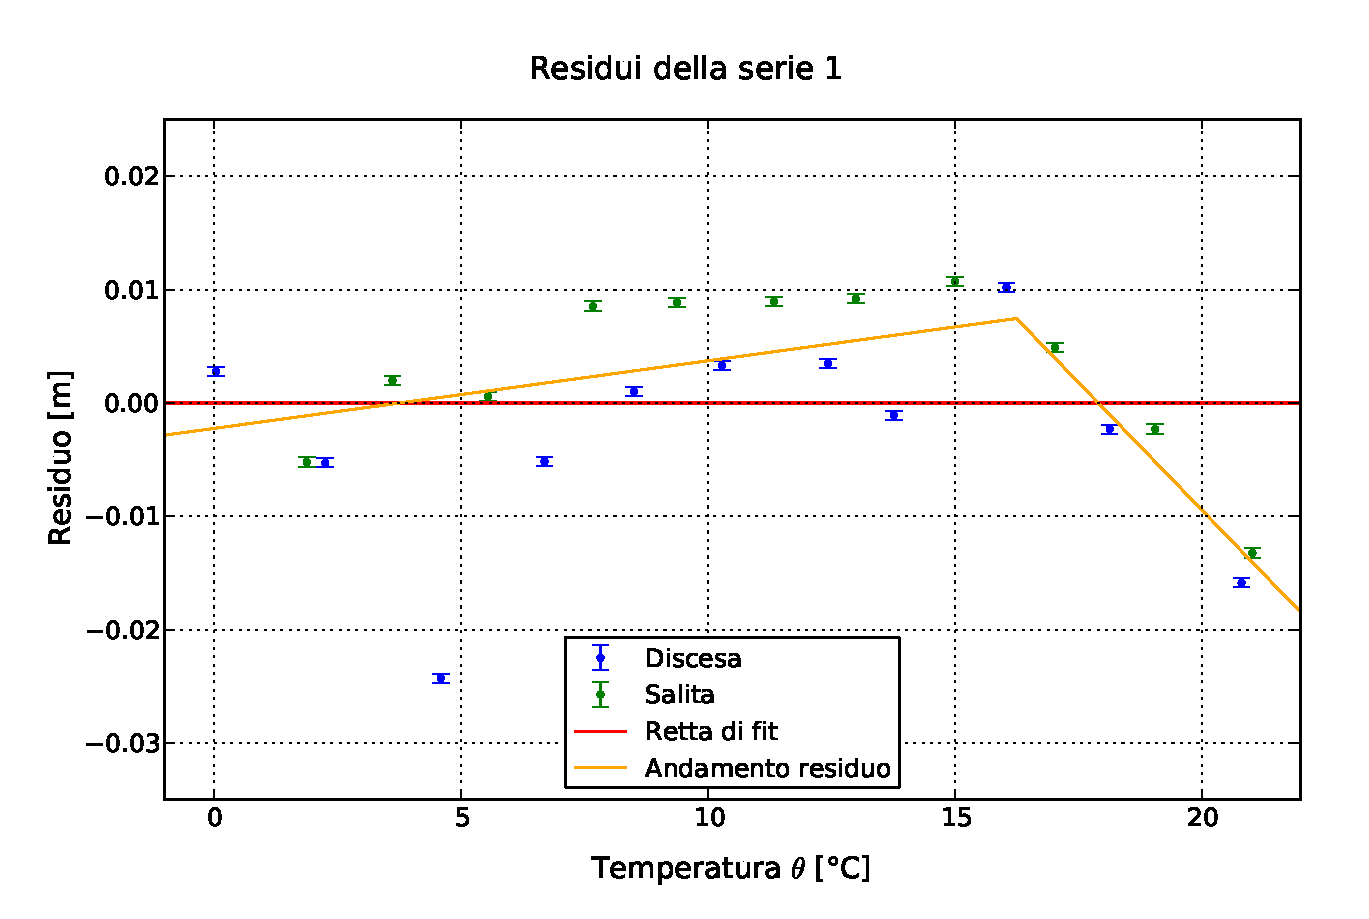
\includegraphics[width=130mm]{immagini/fit1.pdf}
    \caption{Il grafico in figura mostra i residui del fit sulla prima serie di dati. Sono riportati in colori
    diversi i dati presi abbassando (discesa) la temperatura e alzandola (salita). È evidente un andamento residuo nei dati,
    indicato approssimativamente in figura, probabilmente dovuto alla condensazione del vapor acqueo nella bottiglia. L'andamento
    residuo è formato da due rette che si incontrano attorno ai \SI{15}{\celsius}. L'ipotesi è che l'andamento residuo sia dovuto alla
    formazione di condensa all'interno del vaso, che rimuovendo molecole di gas dal recipiente, ha fatto abbassare la pressione e modificato
    la proporzionalità tra dislivello (pressione) e temperatura. C'è anche
    un dato con un residuo molto alto, visibile a sinistra della legenda.}
    \label{fig:fit1}
\end{figure}

\begin{figure}[p]
    \centering
    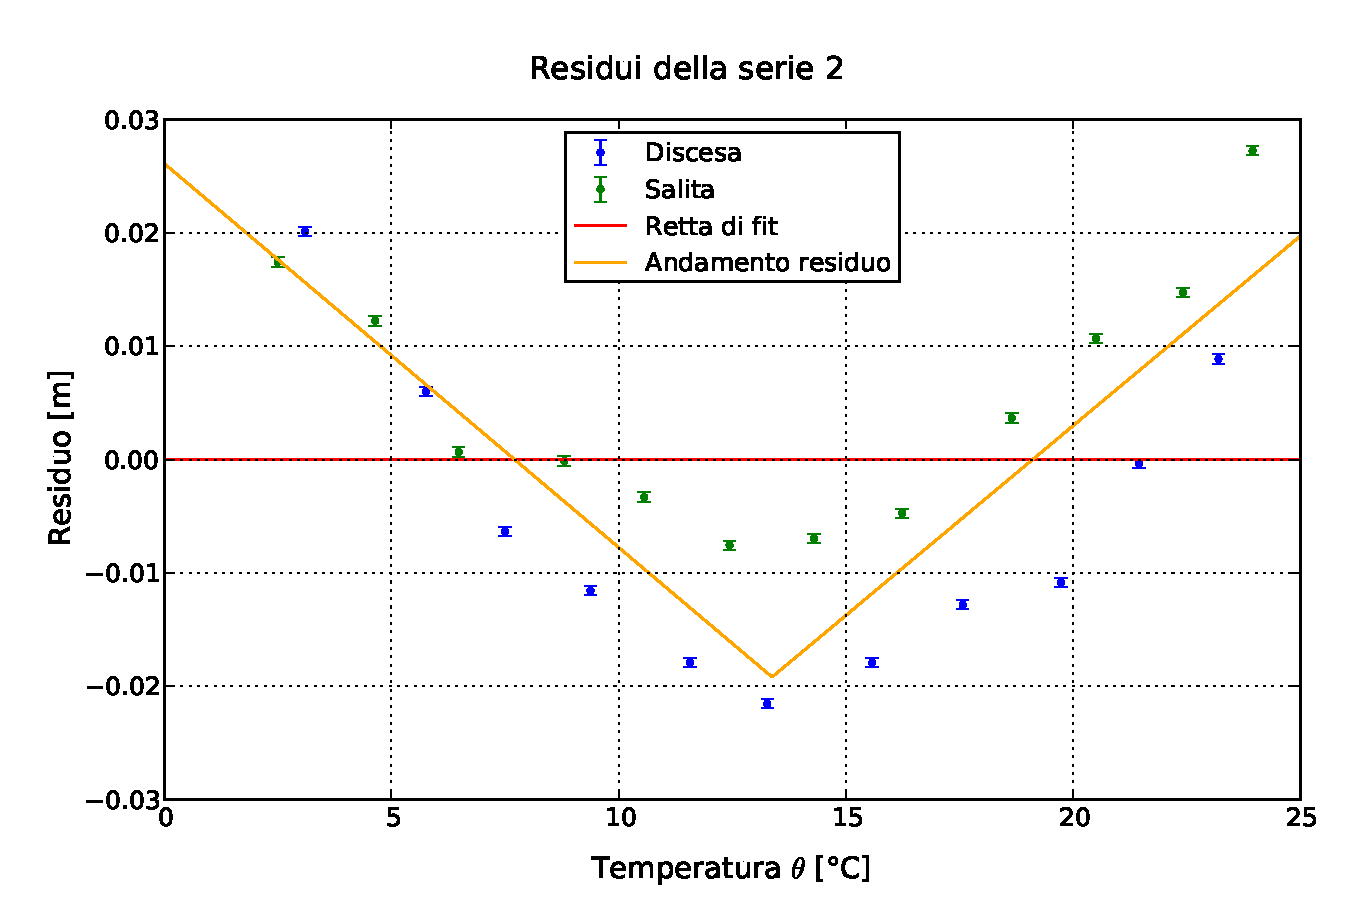
\includegraphics[width=130mm]{immagini/fit2.pdf}
    \caption{}
    \label{fig:fit2}
\end{figure}

Riteniamo quindi che l'errore vada cercato altrove. In figura \ref{fig:fit1} e \ref{fig:fit2} sono riportati i residui delle due
serie di dati. Si notano degli andamenti residui, disegnati nei grafici, che assumono approssimativamente la forma di linea spezzata.
Ci sono stati quindi dei processi, durante l'esecuzione dell'esperimento, che non abbiamo preso in considerazione.
Questo spiega come mai il $\chi^2$ è così alto e perché le incertezze corrette non sono verosimili. I parametri calcolati con
le regressioni precedenti sono privi di senso e anche le rette di fit in realtà sono prive di significato, poiché non
descrivono completamente il fenomeno osservato.
